\chapter{Metode Kembangan}

\section{LSTM Autoencoder}

Long-short term memory (LSTM) neural network adalah arsitektur jenis khusus dari recurrent neural network (RNN) yang dapat mengingat informasi dalam jangka waktu yang panjang.

LSTM cocok untuk mengklasifikasi, memproses, dan memprediksi data time series, karena mungkin terdapat jeda waktu yang tidak diketahui di antara peristiwa penting pada time series.

\begin{figure}[h]
    \centering
    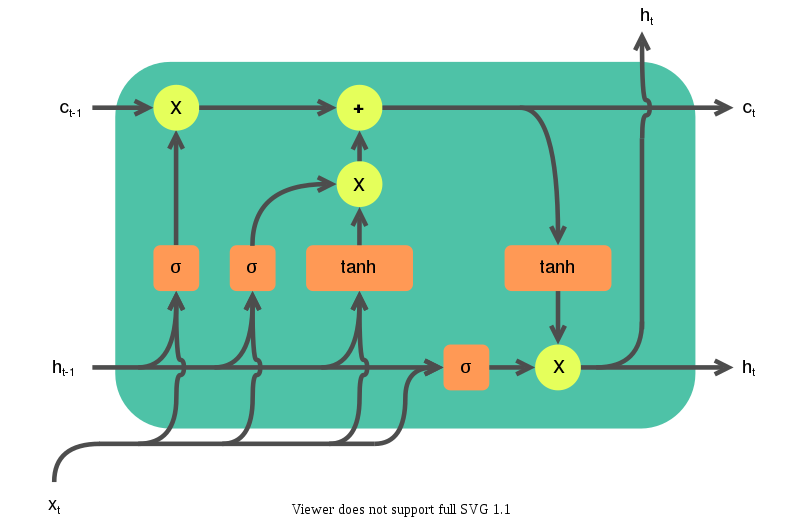
\includegraphics[width=0.8\textwidth]{resources/LSTM/LSTM_cell.png}
    \caption{Satu sel LSTM}
\end{figure}

LSTM Autoencoder adalah model neural network yang menggunakan LSTM sebagai hidden layernya untuk belajar menyalin input ke output. Autoencoder terdiri dari dua bagian, yaitu encoder yang menyalin input menjadi kode dan decoder yang menyalin kode menjadi output.

\begin{figure}[h]
    \centering
    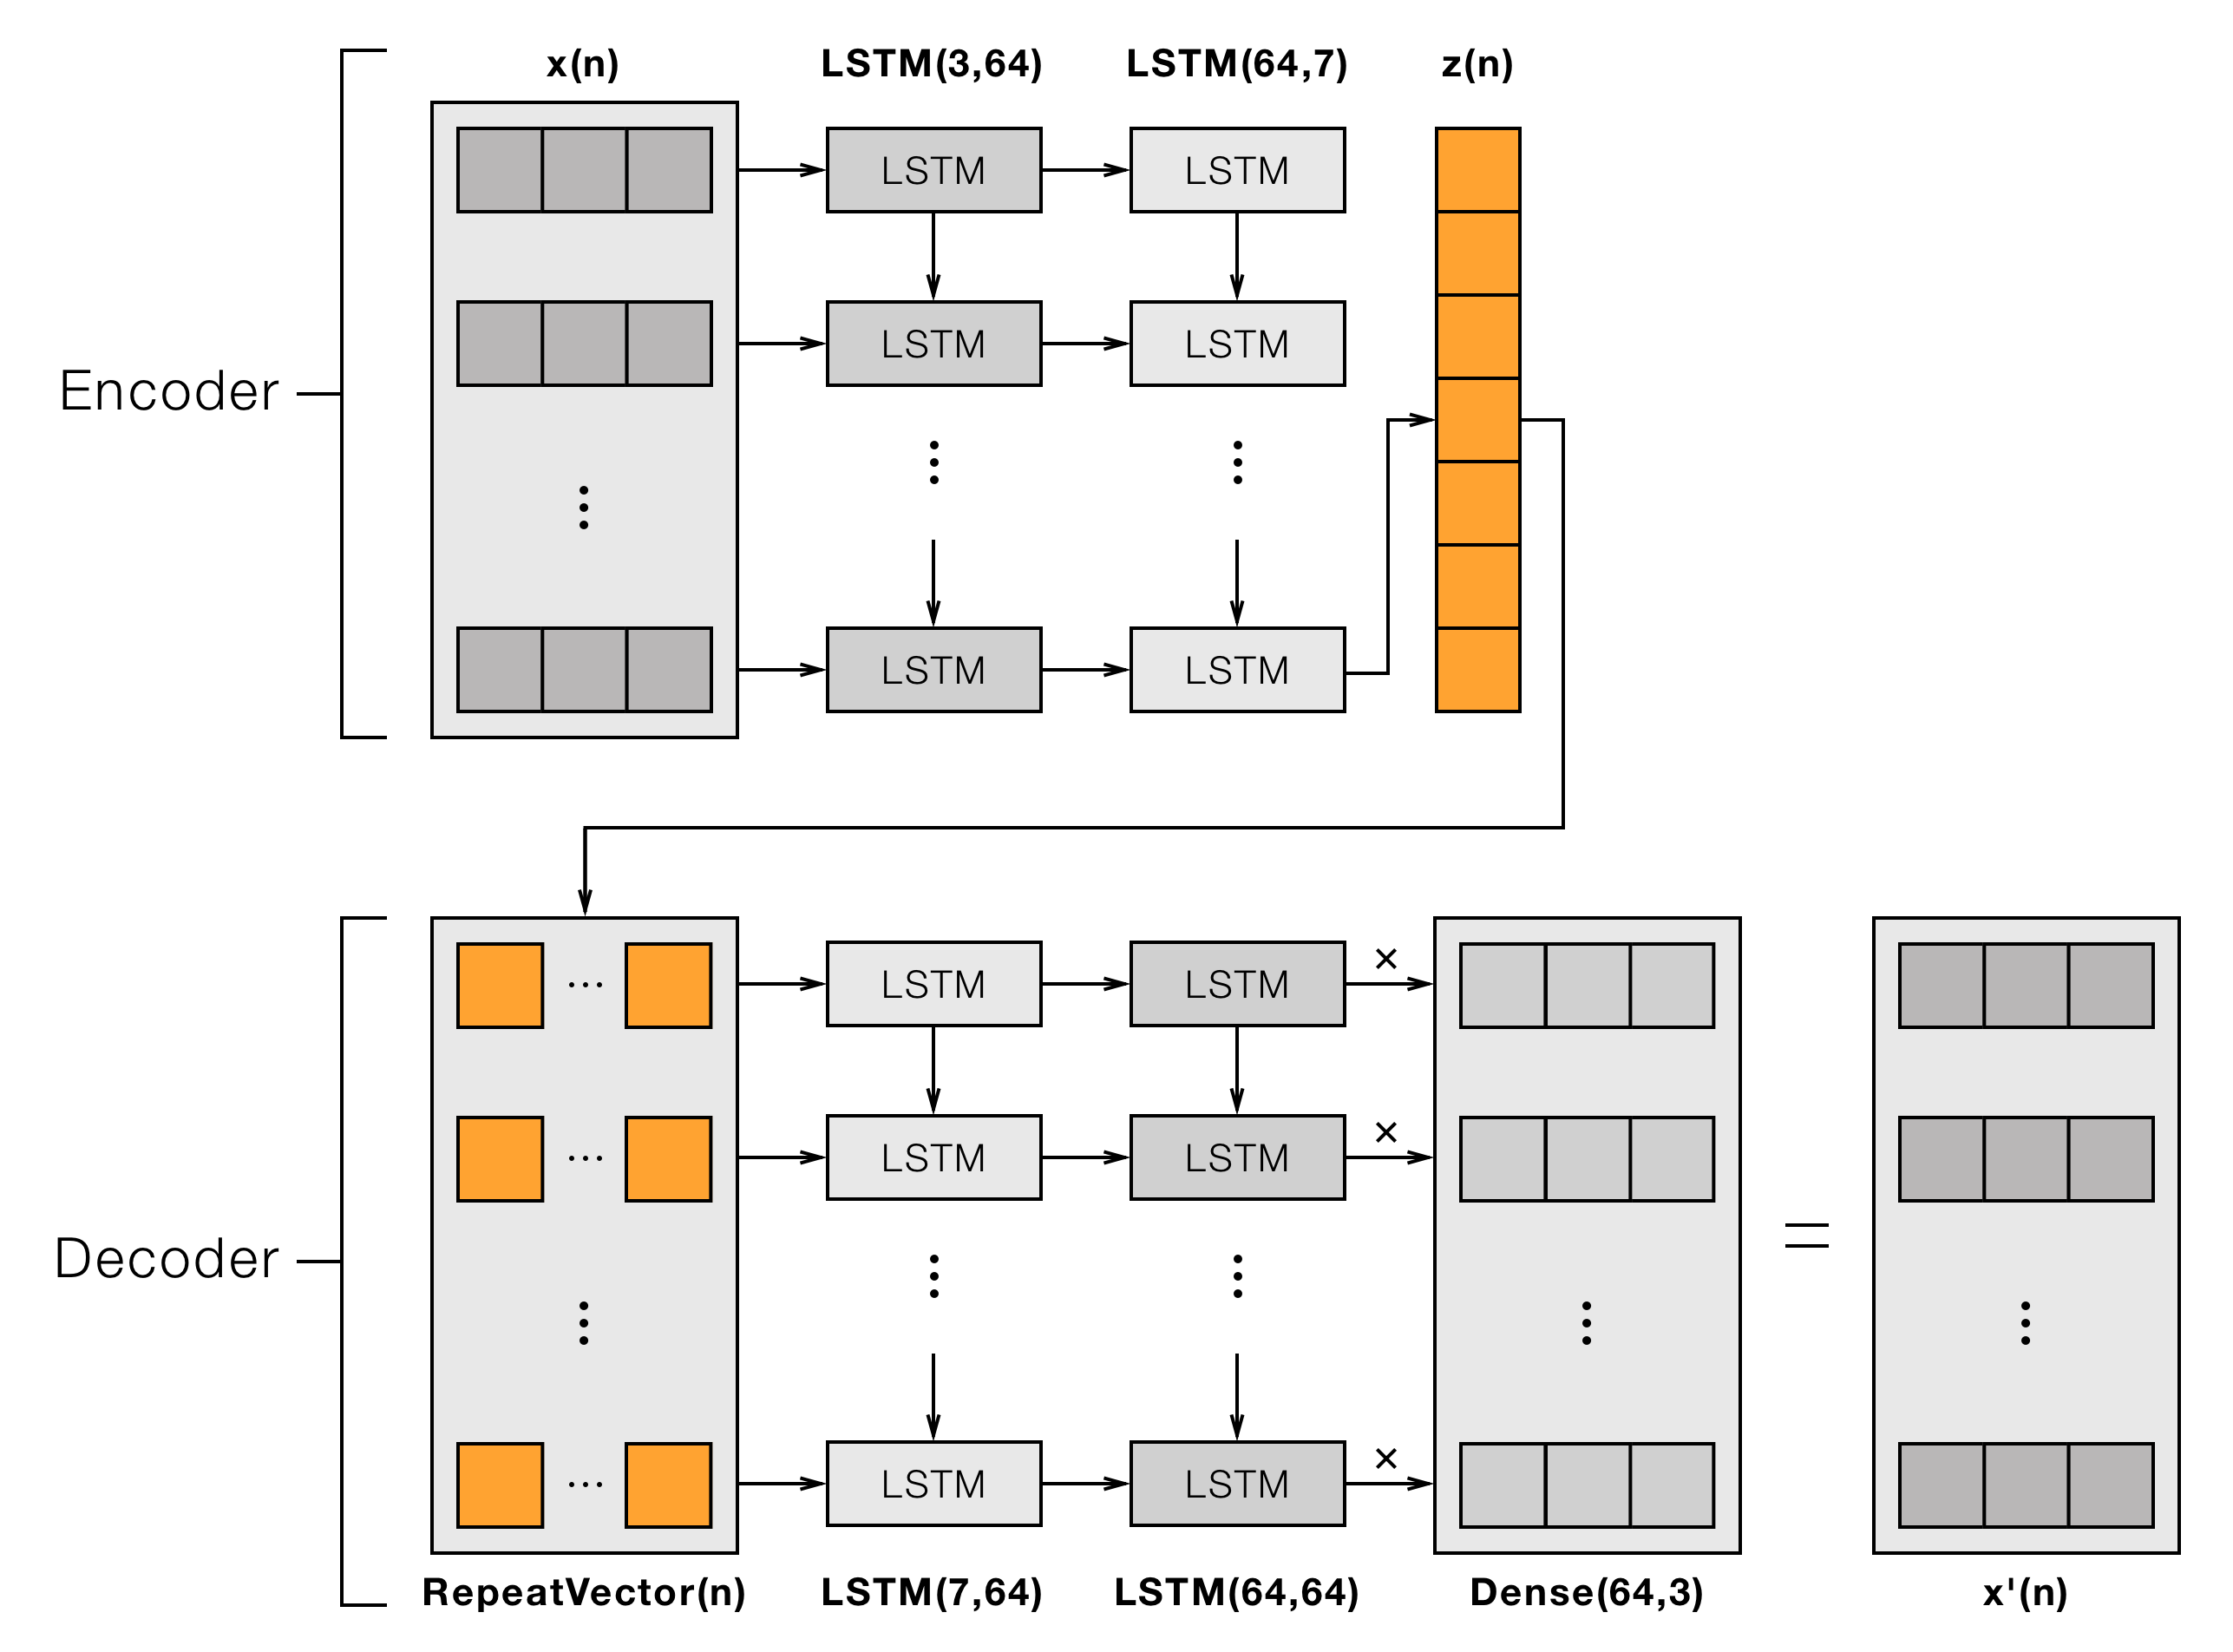
\includegraphics[width=0.8\textwidth]{resources/LSTM/lstm_ae.png}
    \caption{LSTM Autoencoder}
\end{figure}

Dengan begitu autoencoder dapat mempelajari fitur-fitur yang dimiliki input sehingga dapat melakukan prediksi, dan jika menggunakan LSTM sebagai hidden layernya maka dapat digunakan untuk memprediksi input berupa time series.

Karena lebih cocok untuk data time series, maka diharapkan model ini mampu memberikan hasil lebih baik dari model acuan.

\section{Bayesian Probability}

\begin{python}
    time = datetime.datetime.now()
    print("Start training at : {}".format(time))
    
    w = np.zeros(2)
    var_w = 10
    w_iter = []
    w_iter.append(w)
    maxIter = 10
    nIter = 1
    tol = 10**-6
    delta = 10**6
    while (nIter<maxIter) and (delta>tol):
        Hess = H_mat(t,w,X_scaled)
        F_vector = F_vec(t,w,X_scaled)
        dw = np.matmul(np.linalg.inv(Hess),F_vector)
        delta = sum(dw**2)
        w = w - dw
        print("nIter = %d, delta=%.2e"%(nIter,delta))
        w_iter.append(w)
        nIter += 1
    
    time = datetime.datetime.now()
    print("Done training at : {}".format(time))

\end{python}
